\subsection{Diseño Inicial}
El modelo se centra en un \texttt{SistemaDeGestionDePozos} que es el principal de los objetos y el que va a tener en cuenta toda la parametr\'ia dada por los ingenieros para simular el problema.

Este va a almacenar una colecci\'on de \texttt{PlanDeConstruccion} por cada cosa que quiera construir el ingeniero (Planta procesadora, pozo de extracci\'on o tanques de almacenamiento). Tambi\'en se encarga de llevar el \texttt{CatalogoDeExcavadoras} y los \texttt{EventoSobrePozo}, es decir, las extracciones e inyecciones. La l\'ogica de la medici\'on de presi\'on y potencial la extrajimos en un objeto \texttt{CalculadoraDePresion} aparte porque el enunciado ped\'ia que fuera f\'acilmente parametrizable.

Es el sistema quien se encargar\'a de que las construcciones que se deseen hacer sean compatibles con las que ya est\'an en curso, por ejemplo, que no se usen excavadoras que estan siendo utilizadas en otro pozo, y que las extracciones y reinyecciones sean v\'alidas (sobre pozos que est\'en terminados, que la planta procesadora tambi\'en lo est\'e y haya tanques donde almacenar lo extra\'ido, que no se extraiga un d\'ia si hay una reinyecci\'on, entre otros).

Teniendo as\'i un sistema con una colecci\'on de planes de construcci\'on y eventos sobre pozos v\'alidos, se pueden ordenar por fecha y facilmente loguearlo en un archivo.

Tambi\'en puede llevar como par\'ametro el costo de un litro de agua, de gas y combustible para estimar el valor de inyectar agua comprada, de vender gas y el alquiler total de una excavadora, respectivamente.

El objeto \texttt{CalculadoraDePresion} se va a encargar de consultarle al sistema qu\'e pozos est\'an habilitados en un d\'ia, y cuales fueron los eventos hasta ese momento para calcular la presi\'on y el potencial.

Cada \texttt{PlanDeConstruccion} conoce el bien material que est\'a construyendo y una fecha de inicio que es definido por el usuario. Es para los pozos que adem\'as es necesario indicarle qu\'e excavadora usar. Dados los requerimientos, se puede considerar que el sistema busque en el cat\'alogo qu\'e excavadora est\'a disponible en la fecha que se quiere construir y simule la construcci\'on con esa.

Los atributos del resto de los objetos \texttt{PlantaProcesadora}, \texttt{PozoDeExtraccion}, \texttt{ParcelaDeYacimiento}, \texttt{Yacimiento} y \texttt{MantoGeologico} son f\'acilmente entendible apartir del diagrama de clases:

\begin{figure}[H]
  \centering
  \hspace{-3.5cm}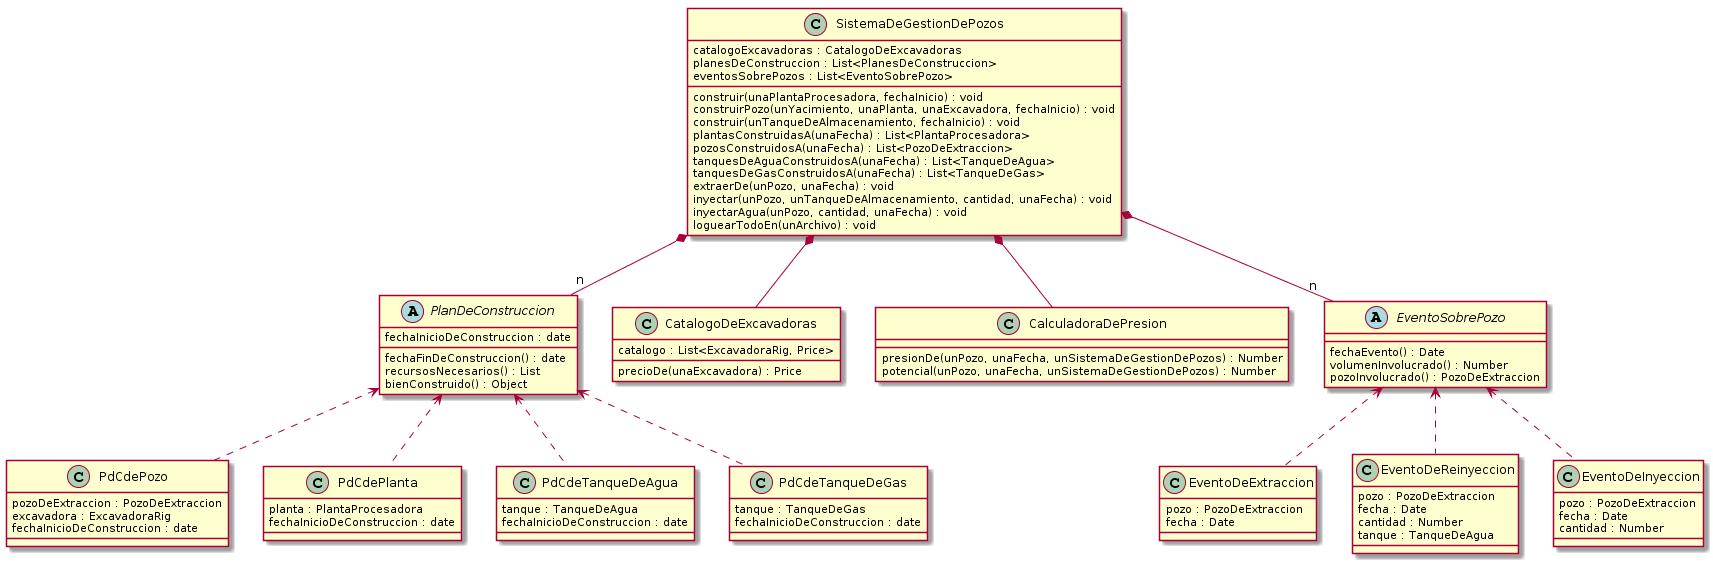
\includegraphics[angle=90,scale=0.4]{Partes/Imagenes/diagrama_alternativo1.png}
    \caption{Diagrama de clases de la construcción de los edificios y el estado de los pozos.}
    \label{fig:dia_cla_gestion_1_1}
\end{figure}

\begin{figure}[H]
  \centering
  \hspace{-3.5cm}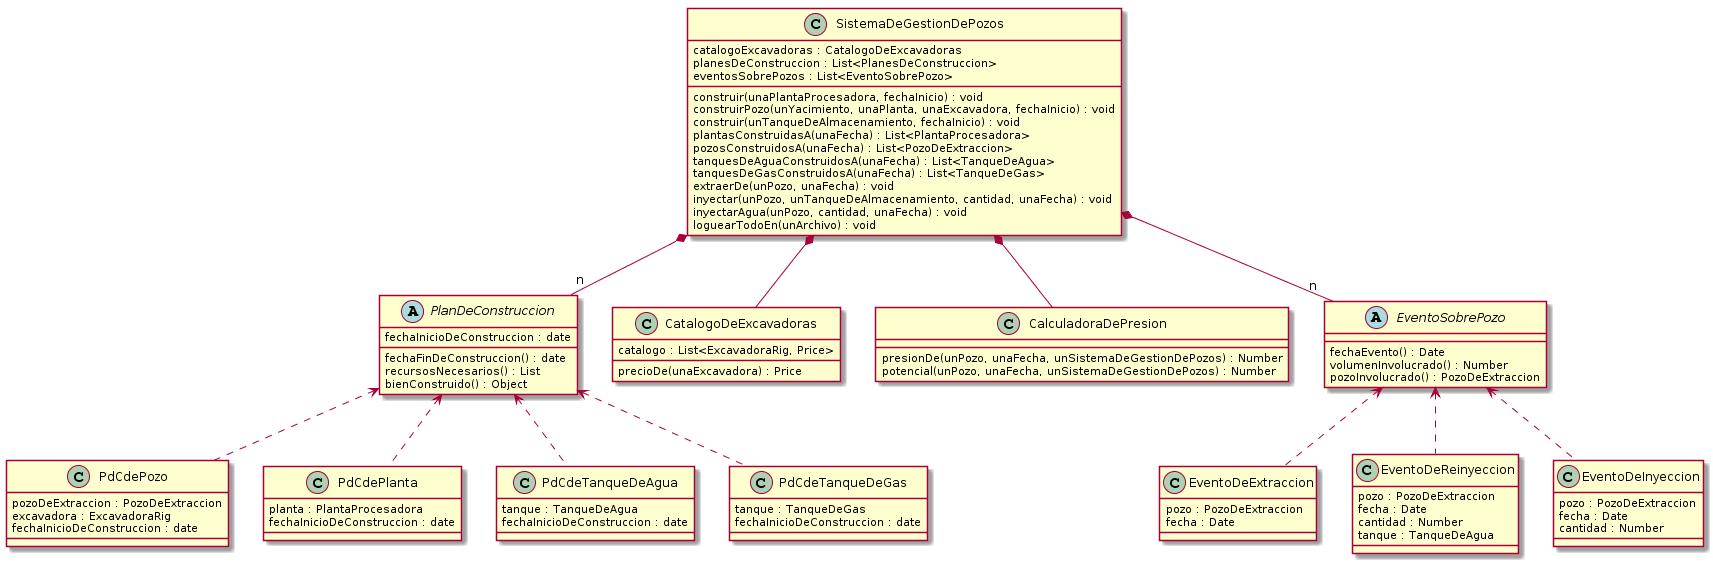
\includegraphics[angle=90,scale=0.35]{Partes/Imagenes/diagrama_alternativo1.png}
    \caption{Diagrama de clases que muestra el diseño de la construcción de los pozos y como se consulta su estado.}
    \label{fig:dia_cla_const_1_1}
\end{figure}
